\section*{Questions 5 and 6}

We now begin to look at the model checker, using the result from Mandatory Assignment 2. Firstly we need a context free grammar which produces the transition system. These productions are seen in table \ref{tab:Q5prod}. Again the first production is in order to read the whole file before parsing. The value "$\epsilon$" is not written in antlr but shown to emphasise that nothing is produced.

\begin{table}[H]
    \centering
    \begin{tabular}{|rl|}
    \hline
    SYS $\;\rightarrow$ & STS \\
    STS  $\;\rightarrow$ & ST $|$ ST STS $|$ $\epsilon$ \\
    ST  $\;\rightarrow$ & '\{' STI '$[$' APS '$]$' ES '$\}$' \\
    STI $\;\rightarrow$ & S $|$ S '*' \\
    APS $\;\rightarrow$ & A $|$ A ',' APS $|$ $\epsilon$ \\
    A $\;\rightarrow$ & P \\
    ES $\;\rightarrow$ & E $|$ E ES $|$ $\epsilon$ \\
    E $\;\rightarrow$ & S \\
    \hline
    \end{tabular}
    \caption{The productions for building the transition system for the model checker. The variable names are again acronymes for the names used in the code: SYS: system, STS: states, ST: state, STI: state\_info, APS: atom\_props, A: atom, ES: edges, E: edge. S is state number and P is an atomic proposition.}
    \label{tab:Q5prod}
\end{table}

This way the transition system is build from zero or more states, following the pattern: 
\begin{gather*}
    ( \: '\{' \: S('*')? \: '[' \: P* \: ']' \: S* \: '\}' \: )*
\end{gather*}

To create the abstract syntax tree, some standard java classes are used together with three new classes: \texttt{State}, \texttt{StateInfo} and \texttt{TransitionSystem}. 

\texttt{StateInfo} is simply an auxillary class to specify if the state is an initial state or not. The \texttt{TransitionSystem} contains a list of \texttt{State}'s, which forms the wanted system. As seen in the productions, the \texttt{State} class has information about initial state, atomic propositions, edges/edge targets, and the state number (also a boolean used when performing ctl checks).

The complete code for the transition system as implemented in antlr3.5 can be seen in the appendix, but the main flow of the parser is summarized in the list below:

\begin{itemize}
    \item The \texttt{system} rule creates the transition system based on a list of states.
    \item The \texttt{states} rule creates the list of states based on each state. 
    \item The \texttt{state} rule creates the state based on the state information. 
    \item The \texttt{state\_info} creates a state\_info based in the state number and if the state is an initial state. 
    \item The \texttt{atom\_props} rule creates a list of strings based on each atomic proposition input.
    \item The \texttt{edges} rule creates a list of integers based on each edge input.
\end{itemize}

To demonstrate that these productions recognizes transition systems with the given pattern, different sets of states are given as input to the program, and the outputs are seen in figures \ref{fig:Q5ex1}, \ref{fig:Q5ex2} and \ref{fig:Q5ex3}.
\begin{figure}[H]
    \centering
    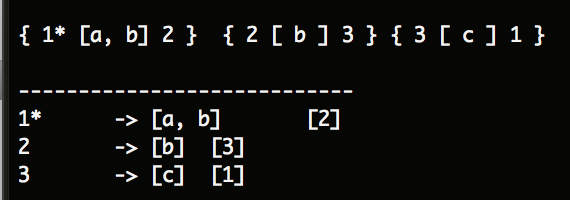
\includegraphics[width=0.4\textwidth]{fig/Q5example1}
    \caption{Transition system with three states, atomic propositions and edge targets.}
    \label{fig:Q5ex1}
\end{figure}
\begin{figure}[H]
    \centering
    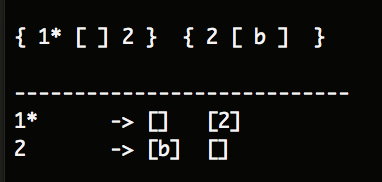
\includegraphics[width=0.3\textwidth]{fig/Q5example2}
    \caption{Transition system with empty atomic propositions or edge targets.}
    \label{fig:Q5ex2}
\end{figure}
\begin{figure}[H]
    \centering
    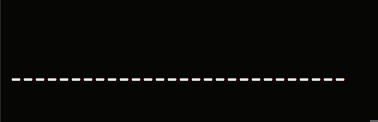
\includegraphics[width=0.3\textwidth]{fig/Q5example3}
    \caption{Empty system with no states.}
    \label{fig:Q5ex3}
\end{figure}
This concludes that the program successfully recognizes the input and builds the abstract syntax tree for the transition system.